\documentclass[a4paper]{article}

% Packages
\usepackage[utf8]{inputenc}
\usepackage{graphicx}
\usepackage{hyperref}
\usepackage{amsmath}
\usepackage{amsfonts}
\usepackage{amssymb}
\usepackage[left=2cm,right=2cm,top=2cm,bottom=2cm]{geometry}
\usepackage{fancyhdr}
\usepackage{glossaries}
\usepackage{listings}
\usepackage{xcolor} % Extended color functionalities
\usepackage{graphicx} % Required for inserting images
\usepackage{tikz}
\usetikzlibrary{automata, positioning, arrows}
\usepackage{float}
\usepackage{subcaption}
\usepackage{wrapfig}


\hypersetup{colorlinks=true, linkcolor=blue}

% Define custom colors
\definecolor{codegreen}{rgb}{0,0.6,0}
\definecolor{codegray}{rgb}{0.5,0.5,0.5}
\definecolor{codepurple}{rgb}{0.58,0,0.82}
\definecolor{backcolour}{rgb}{0.95,0.95,0.92}

% MATLAB style for highlighting
\lstdefinestyle{mystyle}{
    backgroundcolor=\color{backcolour},   
    commentstyle=\color{codegreen},
    keywordstyle=\color{magenta},
    numberstyle=\tiny\color{codegray},
    stringstyle=\color{codepurple},
    basicstyle=\ttfamily\footnotesize,
    breakatwhitespace=false,         
    breaklines=true,                 
    captionpos=b,                    
    keepspaces=true,                 
    numbers=left,                    
    numbersep=5pt,                  
    showspaces=false,                
    showstringspaces=false,
    showtabs=false,                  
    tabsize=2
}

\lstset{style=mystyle}

% Glossary entries
\newacronym{pep}{PEP}{Peak Envelope Power}
\newacronym{papr}{PAPR}{Peak to Average Power Ratio}
\newacronym{ofdm}{OFDM}{Orthogonal Frequency Division Multiplexing}

% Document
\begin{document}

\begin{titlepage}
    \begin{center}
        \vspace*{1cm}

        \Huge
        \textbf{Modulation Waveforms Lab Report}

        \vspace{0.5cm}
        \LARGE
        EXPERIMENT CP-SRP
        EE20017
        
        \vspace{1.5cm}

        \textbf{Jake Stewart}\\
        \textbf{JS3910}\\

        \textbf{Eugene Levinson}\\
        \textbf{EL769}\\
        \vspace{0.8cm}

                \vfill
                
\includegraphics[width=0.5\textwidth]{university_logo.png}

                \Large
                Electrical and Electronic Engineering\\
                University of Bath\\
                United Kingdom\\
                \today
                

            \end{center}
        \end{titlepage}

        \newpage
        \tableofcontents
        \newpage

        \section{Introduction}
        In this report the results of the "Modulation Waveforms" laboratory from the "EE20017 Communication principles module" are presented, discussed and analysed. The goal of the laboratory was to experiment and experience AM modulation and related signal processing using Matlab.

        \section{Modulation Tests}
        A square wave and triangle wave were generated and modulated using the AM\_2.m file provided. To generate the required waveforms as specified in the lab script modulation parameters such as amplitude, frequency and phase were adjusted in the script, to match values specified in the script. Other parameters such as load resistance and loss were checked and adjusted if needed.

        The script provided generates plots that are a very helpful visualization and can also be used to perform signal analysis and calculations. However since all data is already available through Matlab, all further analysis was done by adding extra calculations steps to the Matlab scripts.

        The following code was used to calculate \gls{pep} and \gls{papr}:

        \begin{lstlisting}[language=Matlab, caption={Signal processing calculations}, label={lst:singnalcalcs}]
            % AM Power
            R = 50; % Ohms
            AM_Power = (AM_time.^2) / (2*R); % RMS Power in Watts V^2/2R
            % Peak Envelope Power
            PEP = max(AM_Power)
            % Peak to Average Power Ratio
            PAPR = PEP/mean(AM_Power)
        \end{lstlisting}

        \subsection{Results}
        \subsection*{Square Wave}
            The carrier signal was modulated with the the waveform approximating a square wave using the provided script and modulation parameters.
            \\\\
            To calculate the \gls{pep}, formula can be used: $PEP = \frac{(\frac{V_{peak}}{\sqrt{2}})^2}{R}$. Where $V_{peak}$ is the maximum absolute value of the wave's amplitude. This was done in Matlab by running a element wise operation to calculate power for each sample point in the modulated signal and then finding the maximum (see Listing \ref{lst:singnalcalcs}).
            \\\\
            To calculate the mean power the following equation can be used: $P_{\text{mean}} = \frac{V_c^2}{2R} + \sum_{i=1}^{n} \frac{V_{m_i}^2}{2R}$ where

            \begin{itemize}
                \item \( P_{\text{mean}} \) is the mean power of the AM wave.
                \item \( V_c \) is the RMS voltage of the carrier signal.
                \item \( V_{m_i} \) is the RMS voltage of each modulation signal.
                \item \( R \) is the resistance of the load.
                \item \( n \) is the number of modulation frequencies.
            \end{itemize}
                
            Finally \gls{papr} can be calculated using : $PAPR = \frac{PEP}{P_{mean}}$

            The following results were obtained: 
                
        \begin{itemize}
            \item $PEP$: 214.7 mW
            \item $P_{mean}$: 45.4 mW
            \item $PAPR$: 4.7312
        \end{itemize}

        The following powers (in mW) were observed on the AM spectrum plot: $14.4000$, $3.6000$, $0.3992$, $0.1440$ for $f_c$, $f_{m1}$, $f_{m2}$, $f_{m3}$ respectively (Figure 1). The side bands account for 28.47\% of the power.

        No cross over distortion was observed. When inspected the modulated signal appears to be smooth with no apparent distortion. There are no signs of the signal being modulated bellow 0 (Figure 2). This is further backed up by the fact that the FFT plot shows no unexpected harmonics

        \begin{figure}[htbp]
        \centering

        \includegraphics[width=0.5\textwidth]{Images/AM_RX_1/Square Wave/AM Spectrum.jpg}
        \caption{AM Spectrum of square modulated signal (excluding mirror frequencies)}

        \end{figure}

        \begin{figure}[htbp]
        \centering

        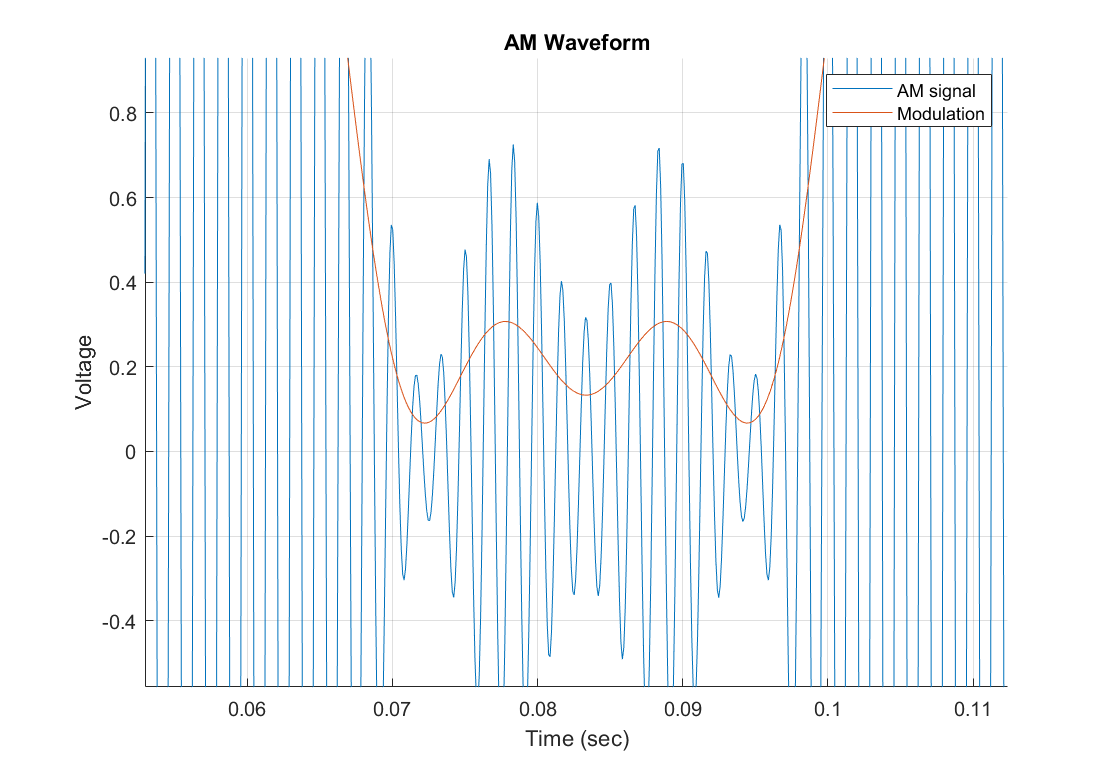
\includegraphics[width=0.5\textwidth]{Images/AM_RX_1/Square Wave/No Distortion.png}
        \caption{AM and modulation signal showing no distortion}

        \end{figure}

        \newpage

        \subsection*{Triangular Wave}
        The parameters of the modulation signal were adjusted according to the lab script to approximate a triangle wave. The same approach as the one used for the square wave was used to calculate $PEP$ and $PAPR$.

        \noindent

        \begin{itemize}
            \item ${PEP}$: 369.6 mW
            \item ${PAPR}$: 8.14
        \end{itemize}

        The same powers as for the square wave (in mW) were observed on the AM spectrum plot: $14.4000$, $3.6000$, $0.3992$, $0.1440$ for $f_c$, $f_{m1}$, $f_{m2}$, $f_{m3}$ respectively (Figure 3). The side bands account for 28.47\% of the power.

        No cross over distortion was observed in this modulation either. When inspected the modulated signal appears to be smooth with no apparent distortion and no unexpected harmonics in the FFT plot (Figure 5).

        \begin{figure}[htbp]
        \centering

        \includegraphics[width=0.5\textwidth]{Images/AM_RX_1/Triangular Wave/AM Spectrum.jpg}
        \caption{AM Spectrum triangle modulated signal (excluding mirror frequencies)}

        \end{figure}

        \begin{figure}[htbp]
        \centering

        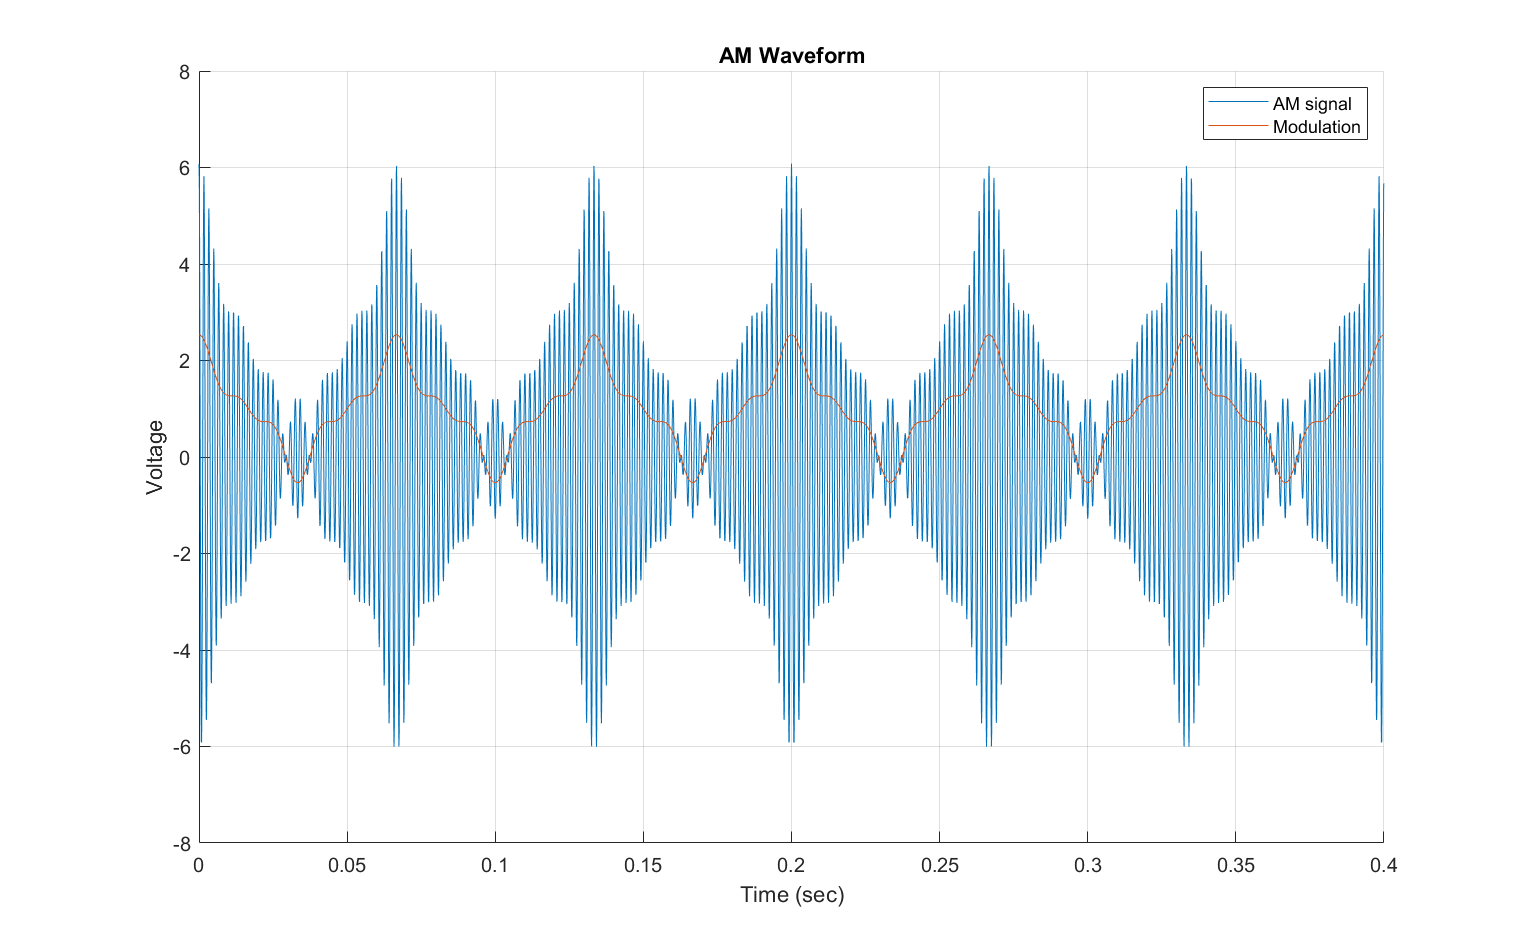
\includegraphics[width=0.5\textwidth]{Images/AM_RX_1/Triangular Wave/Full AM.png}
        \caption{AM and modulation signal (triangle)}

        \end{figure}

        \begin{figure}[htbp]
        \centering
        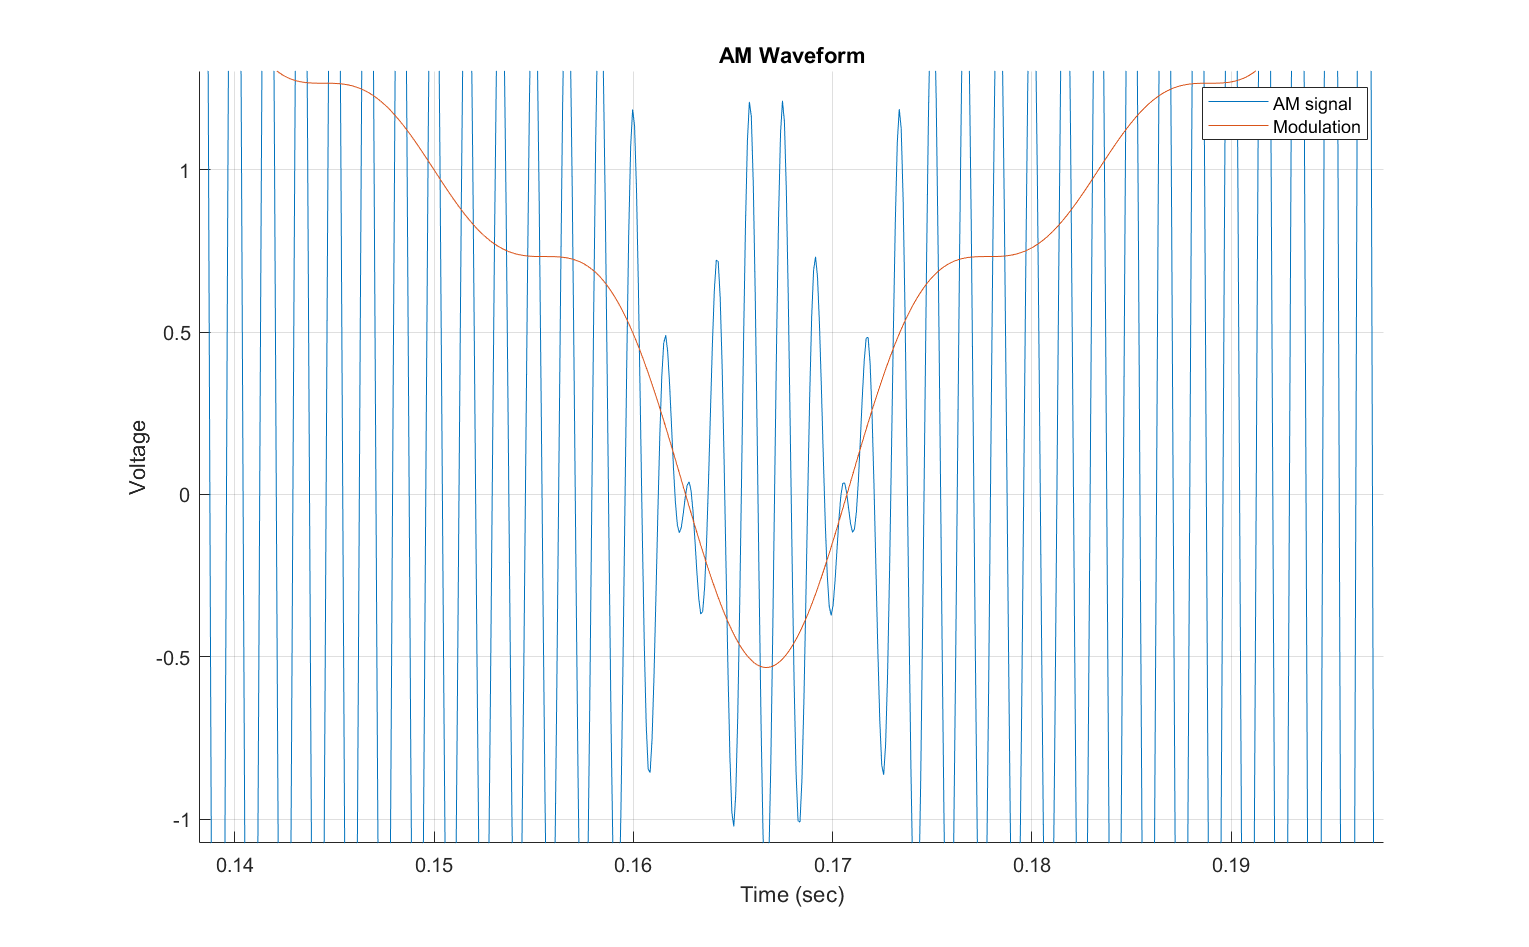
\includegraphics[width=0.5\textwidth]{Images/AM_RX_1/Triangular Wave/Zoomed.png}
        \caption{AM and modulated signal showing no distortion}

        \end{figure}


        \section{Demodulation/detection}

        \subsection{AM detection}
        The "AM\_RX\_1.m" was configured according to the modulation table provided in the lab script. Observing the waveform it can be seen that they follow the input modulation very well. There is no noticeable distortion, or clipping or over modulation. The $o_S$ signal has a significantly higher amplitude due to have been multi9plied by the carrier during modulation (Figure 6). All signals are in phase.

        \begin{figure}[htbp]
        \centering

        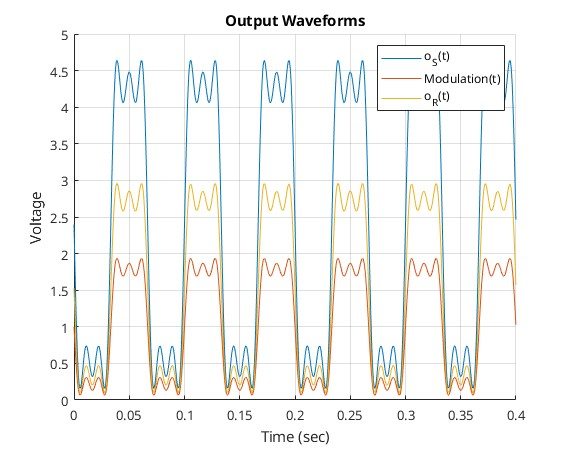
\includegraphics[width=0.5\textwidth]{Images/AM_RX_1/Square Wave/Output Waveforms.jpg}
        \caption{RX outputs comparison}

        \end{figure}

        \begin{figure}[htbp]
        \centering

        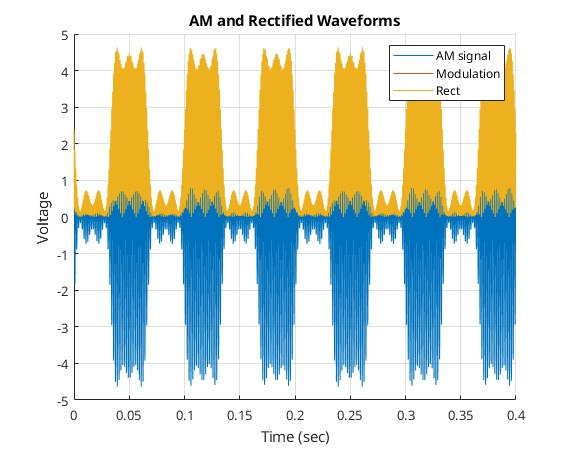
\includegraphics[width=0.5\textwidth]{Images/AM_RX_1/Square Wave/AM and Rectified Waveforms.jpg}
        \caption{AM and rectified waveform}

        \end{figure}

        \newpage

        The waveform parameters were then changed to modulate using a triangle wave approximation. Almost identical behaviour is observed with no distortion or clipping or phase shifts. However there is one key difference - the effects of rectification are clearly seen on the $o_R$ signal. We can see the negative components being mirrored into the positive half (Figure 8).

        \begin{figure}[htbp]
        \centering

        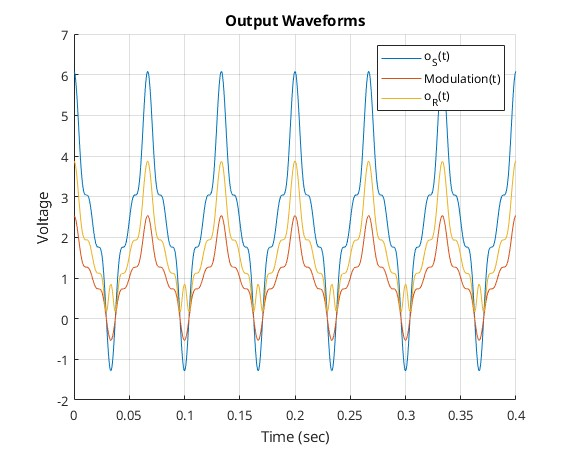
\includegraphics[width=0.5\textwidth]{Images/AM_RX_1/Triangular Wave/Output Waveforms.jpg}
        \caption{RX output comparison for triangle modulation}

        \end{figure}

        \newpage



        \subsection*{Phase offset in receiver carrier}
        The phase of the receiver carrier signal was changed in increments of $\pi/4$. As the phase changes it can be observed that the amplitudes of the demodulated signal change. Most notably the $o_s$ is offset down up to -6V and $o_R$ peak to peak amplitude is reduced.


        \begin{figure}[htbp]
        \centering

        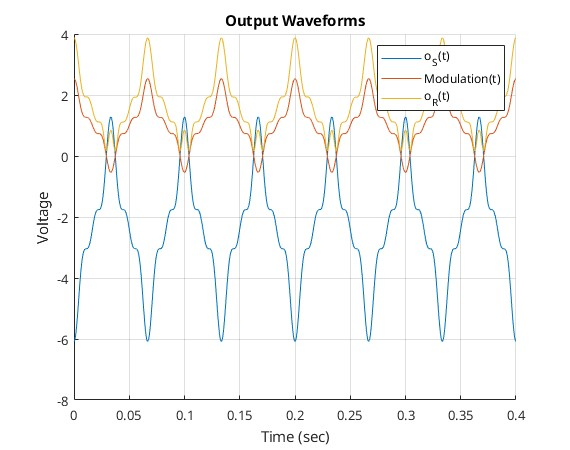
\includegraphics[width=0.5\textwidth]{Images/AM_RX_1/Triangular Wave/Receiver Carrier Phase Offset/Output Waveforms + 4pi 4.jpg}
        \caption{Triangle wave demodulated with receiver carrier phase offset to $4\pi$ }

        \end{figure}

        These changes appear due to the mismatch in phase of the sender and receiver carrier which results in destructive , reducing and shifting the amplitude.


        \subsection*{Frequency offset in receiver carrier}
        The modulation and carrier singals' parameters were set as specified in the lab script. When looking at the two demodulated signals, the $o_R$ is demodulated correctly, with no noticeable distortion (Figure 10). However the $o_S$ is heavily effected. This is because $o_S$ relies on the carrier and receiver carrier matching frequencies, since multiplication by the receiver carrier is performed. If the carrier frequency does not match the receiver carrier, then the effects mimic those of adding more modulation with another signal - the wave form changes drastically. On the other hand the rectified output is not effected as it does not rely on a receiver carrier at all.

        \begin{figure}[htbp]
        \centering

        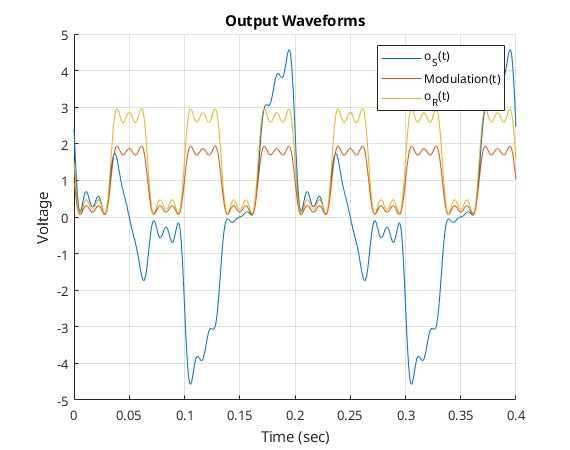
\includegraphics[width=0.5\textwidth]{Images/AM_RX_1/Square Wave/Receiver Carrier Frequency Offset/Output Waveforms.jpg}
        \caption{Square wave with mismatched TX and RX frequencies }

        \end{figure}


        \section{Orthogonal Frequency Division Multiplexing (OFDM)}
        \subsection{OFDM Baseband Signal}
        The parameters in the provided Matlab script were set as per the lab script.
        The following values were calculated:
        \subsection*{"S" Symbol @ 1V}
        \begin{itemize}
            \item ${PEP}$: 41.44W
            \item ${PAPR}$: 8.22
        \end{itemize}

        \subsection*{"S" Symbol @ 2.5V}
        \begin{itemize}
            \item ${PEP}$: 1.8W
            \item ${PAPR}$fair: 8.22
        \end{itemize}

        \subsection{64-QAM on OFDM}
        Matlab was used to calculate PEP and PAPR for each of the following symbols:

        \begin{tabular}{|l|l|l|}
        \hline
        \textbf{Symbols} & \textbf{PEP} & \textbf{PAPR} \\ \hline
        "X" & 141W & 2 \\ \hline
        "+" & 150W & 3.99 \\ \hline
        "Y" & 425W & 3.99 \\ \hline
        "<" & 11.4WW & 3.97 \\ \hline
        "3" & 57.4W & 3.98 \\ \hline
        "X+Y<3" & 1372W & 5.92 \\ \hline
        \end{tabular} \\

        \subsection{Summary and comments}

        AM signals typically rely on envelope detection methods, which may suffer from noise and distortion. For receiving OFDM signals, coherent detection schemes are more suitable due to their ability to handle the complex multipath environment and mitigate inter symbol interference, making them preferable over envelope detection methods used in AM demodulation.

        \end{document}
